\documentclass[journal]{IEEEtran}
%\documentclass[10pt,journal,cspaper,compsoc]{IEEEtran}

%\usepackage{ifpdf}
%\usepackage[nocompress]{cite}
\usepackage{graphicx}
\usepackage{amsthm}
%\usepackage[cmex10]{amsmath}
%\usepackage{amssymb}
\usepackage{caption}
\usepackage[font=scriptsize,,labelfont=sf,textfont=sf]{subfig}
\usepackage{algorithm}
\usepackage{algpseudocode}
%\usepackage{fixltx2e}
%\usepackage{footnote}
%\usepackage{url}
%\usepackage[top=0.8in, bottom=0.7in, left=0.7in, right=0.7in]{geometry}

\hyphenation{op-tical net-works semi-conduc-tor}

\newtheorem{InscribedAngleTheorem}{Theorem}
\newtheorem{IATCorollary}{Corollary}

%\graphicspath{{converted_graphics/}}
\begin{document}

\title{Another On-Line Data Compression Algorithm\\ for Trajectories (OLDCAT)}

\author{Ting~Wang, ~\IEEEmembership{Senior Member,~IACSIT,}
\thanks{Manuscript received Feb 20, 2013. This work was supported in part by the Singapore Economic Development Board (EDB). }
\thanks{Dr. Wang Ting is with SAP Asia Ptd Ltd, Singapore. (E-mail: dean.wang@sap.com)}
}

\maketitle

\begin{abstract}
In the regime of ``Big Data'', data compression techniques take crucial part in preparation phase of data analysis. It is challenging because statistical properties and other characteristics need to be preserved while the size of data need to be reduced. In particular, to compress trajectory data, movement status (such as position, direction, and speed \textit{etc.}) need to be retained. Moreover, for the increasing demand of real-time processing capability, ``online'' algorithms are becoming more desirable in data analysis.  In this paper, we introduce an \emph{OnLine Data Compression Algorithms for Trajectories (OLDCAT)}, which is an elegant, fast algorithm to effectively compress trajectory data to desirable volume. It is able to deal with real-time data, and scalable to adapt to different sensitivity, accuracy, and compression requirements. An evaluation of its parameter settings and a case study are also discussed in this paper. 
\end{abstract}

\begin{IEEEkeywords}
Data Compression, Trajectory Data, Online Algorithm
\end{IEEEkeywords}

\section{Introduction}
Over the last few decades, with the increasingly accurate positioning services (\textit{e.g.} GPS, AIS, Mobile Phone Triangulation, RFID/Wi-Fi tracking \textit{etc.}) and the decreasing price of their deployment, locational data becoming pervasive in our daily lives and scientific researches. Either indoor or outdoor, it is not difficult to obtain the trace, the velocity, and even the acceleration of any moving entity (referred to as an \emph{object} in this paper) of our interest, providing proper equipments and infrastructure. Massive data have been collected in various research projects since early 90�s\cite{tim90ITEJ}. As part of the ``big data regime'', interests in locational data has recently grown even more rapidly thanks to the new database technology and data mining techniques. When locational data coupled with time-stamps, it becomes \emph{spatial-temporal} data --- with both space (spatial) and time (temporal) information  \cite{andrienko2006exploratory}. The timely sequence locations of an object defines its \emph{trajectory}. When multiple objects are concerned, an ID string or number is used in trajectory data for identifying the objects.

Trajectory of objects are widely used in a variety of business and public sector applications, such as traffic modeling and supply chain management \cite{forum2010improving}. These efforts are being hampered by the sparse nature of data collection strategies, the sheer volume of the data, and technical issues associated with the use of the data. The enormous volume of data can easily overwhelm human analysis.  This motivates the need for automated methods to compress and analyze the data. 

There are mainly two different approaches in data compression:
\begin{itemize}
  \item Coding based: data is \emph{encoded} using fewer number of bits than the original representation \cite{wade94signal}. Data will be \emph{decoded} before used in other applications or analysis;
  \item Sampling based: part of the data is taken as \emph{samples} while others are disregarded. Sampled data could be directly used in applications or analysis. However, good sampling algorithms will be needed to preserve statistical properties or other characteristics of the data.
\end{itemize}
While the coding approach is more relevant to data storage and presentations techniques (such as video and audio compression and streaming), sampling based compression is more commonly used with data obtained from measurements or signals, such as trajectory data. In this paper, we will focus on the sampling based approach, \textit{i.e.} on how to sample trajectory data efficiently and effectively.

In computer science, an \emph{online algorithm} \cite{Azar98OLB} is one that can process its input piece-by-piece in a serial fashion, \textit{i.e.}, in the order that the input is fed to the algorithm, without having the entire input available from the start. In contrast, an \emph{offline} algorithm is given the whole problem data from the beginning and is required to output an answer which solves the problem at hand. In the context of trajectory data mining, online algorithms are extremely useful to enable real time configurations and optimizations. For example, to use the GPS data of the vehicles in traffic management, online algorithms should be preferred, as we could not wait till the end of the day to study the traffic pattern. Congestion and accidents would only be prevented or reduced if we were able to make online (real-time) adjustment to the policies (\textit{e.g.} traffic lights, route recommendations). Data compression, as part of the data mining process, will also need to be online to deal with real-time, streaming data. Moreover, simple, fast yet elegant algorithms will be desirable so that more time and computational resources could be used on more tedious tasks (such as the classification and optimization problems). 

In this paper, we propose an \emph{On-Line Data Compression Algorithm for Trajectories (OLDCAT)}. It deals with the trajectory sampling and compression problem; identifies key points in a trajectory that define its characters; and re-constructs the trajectory with much fewer data points. A brief introduction to the existing works and challenges are discussed in Sect.~\ref{sect:exist}, followed by our discussion of the OLDCAT algorithm in Sect.~\ref{sect:algo}. We also show that by adjusting the parameters of OLDCAT, accuracy and scale of the compression is flexible and predictable in Sect.~\ref{sect:anal}. A case study of how OLDCAT could be used with some harbor data is discussed in Sect.~\ref{sect:case}. Sect.~\ref{sect:con} concludes the paper with our findings and contributions.


\section{Existing Works and Challenges}
\label{sect:exist}
Based on dynamic programming, Bellman's algorithm \cite{Bell61ACL, Bell03DP} has over 50 years of history in using point samples to represent lines and curves. Its results have been proven optimal with minimal root mean square errors under given conditions. The original implementation of this algorithm has a worst-case running time of $O\left(n^3\right)$, where $n$ is the number of points in the trajectory. This is a serious drawback that stops it being used with large data set or when real-time solution is required. A recent update \cite{klein06ad} shows with additional storage, the running time of Bellman's algorithm could be reduced to $O\left(n^2\right)$. However, it still not fit to the ``online'' requirement, and not able to deal with really ``big'' data.

The Douglas-Peucker algorithm \cite{doug73algo} is the all-time classic line generalization heuristic. It is commonly used to represent a curve with a series of line segments, and thereby compress the storage requirement. However, as pointed out by Meratnia and de By in \cite{Mera04EDBT}, Douglas-Peucker algorithm and its other implementations are not suitable for trajectory data as they could not deal with the time information, and may have treat the locational data in wrong sequence. Meratnian and de By thus proposed their own algorithm namely \emph{Top-Down Time Ratio (TD-TR)} algorithm, which utilizes the temporal component in the trajectory data. Based on TD-TR, they extended their works to \emph{OPen Window Time Ratio (OPW-TR)} and \emph{OPen Window SPatial-temporal (OPW-SP)} algorithms, which are similar to TD-TR but use different windowing criteria and error-thresholds. The majordraw back of this group of algorithms is that they requires all the trajectory data be available before choosing the line segments that represent the trajectory. Therefore they are ``offline'' solutions to the problem we are looking at.

The \emph{STTrace} algorithm \cite{pot06SSDM} is capable of dealing with online trajectory data streams, but it also requires object heading and speed information to characterize a trace. Similarly, the \emph{Semantic Trajectory Compression} \cite{schmid09ASTD} algorithm uses urban map together with GPS data. The additional information (\textit{e.g.} speed, heading, or map) may not be always available with the trajectory data, and thus the suitable scope of these algorithms are limited. In our work, we aim to compress the trajectory with minimum information, \textit{i.e.} the object ID, the time stamp and the longitude/latitude values from any positioning service. 

Another challenge in trajectory data compression is that due to signal interference or technical flaw, data may not be accurate. For example, it's normal to have $\sim 10$m error in GPS data. For mobile phone triangulation, error can go as high as 1 mile when base stations are scarcely located. Even in a tiny city such as Singapore, the error is $\sim 2$m on average. Effective compression algorithms need to be able to deal with such error/noise in the raw trajectory data. 

Moreover, scalability is another desired feature in trajectory studies. One may want to understand the ``big picture'' of the trajectory as well as details of movements in some particular areas. This means we should be able to view different levels of details when needed, by adjusting the parameters of the algorithm. We will show in the next section how we make our On-Line Data Compression Algorithm for Trajectories, \textit{a.k.a.} OLDCAT be online, adaptive, and scalable. 

\section{The OLDCAT}
\label{sect:algo}
As discussed in the previous section, we assume only minimum information in the raw data: the object ID, time stamp $t$, and longitude/latitude values $\left(x,y\right)$. For the convenience of discussion, we focus on a single object. The same algorithm and related discussion can easily be extend to the cases of multiple objects. 

We assume the raw data stream consists of a series locational data with time stamps, denoted as 
\[
\mathcal P = \left\{ P_{t_0}, P_{t_1}, P_{t_2}, \dots, P_{t_n},\dots\right\}, 
\]
where $P_{t_n} = \left(x, y, t_n\right)$ is referred to as a \textit{data point}. The objective of OLDCAT is to find a sampled subset of $\mathcal P$ denoted as $\mathcal P' \subset \mathcal P$ and
\[
\mathcal P' = \left\{ P_{t_0}, P_{t_i}, P_{t_j}, \dots\right\}_{0<i<j}, 
\]
to represent $\mathcal P$. 

We note that the raw data stream may not be continuous, as the signal may disappear when the positioning device is switched off or out of reach. Also, the object may stop moving from time to time. These events breaks the trajectory into \emph{segments}. We define 5 different types of points that construct a trajectory:
\begin{description}
  \item[STAY Point]\hfill \\ where the object stops moving and remain stationary for a period longer than a predefined constant $T_{\rm{max}}$. A STAY point itself forms a trajectory segment. Denoted as $\mathbf S$. 
  \item[BEGIN Point]\hfill \\ where a segment of trajectory begins. It marks the location where the signal of the object appears after disappeared for a period of length $T_{\rm{max}}$, or the object moves off from a stay point for a distance longer than $D_{\rm{min}}$. This minimum distance control parameter $D_{\rm{min}}$ is needed to tolerate signal noises and errors. MOVE points are denoted as $\mathbf B$. 
  \item[END Point]\hfill \\ where a segment of trajectory ends, when signal fades out or object stops moving. A BEGIN point together with the following next END point define a segment of the trajectory. Denoted as $\mathbf E$. 
  \item[MOVE Point]\hfill \\ where the object moves forward with out making significant turns for a distance longer than a predefined constant $D_{\rm{max}}$. Denoted as $\mathbf M$. 
  \item[TURN Point]\hfill \\ where the object turns for an angle sharper than a predefined value $\Theta_{\rm{min}}$. Denoted as $\mathbf T$. 
\end{description} 
We use $\leftarrow$ to denote the state of $P$. For example, $P \leftarrow \mathbf S$ means $P$ is of type STAY. The parameters ($D_{\rm{max}}$, $D_{\rm{min}}$, $T_{\rm{max}}$, $\Theta_{\rm{min}}$) can be adjust to according to the requirement of the trajectory data or the signal quality. This will be discussed in detail in Sect.~\ref{sect:anal}. 

When a new data point $P_t$ is collected, OLDCAT tries to identify whether it belongs to one of the 5 types above. If yes, we will add $P_t$ to $\mathcal P'$, otherwise the data point will be disregarded. In the following section, we describe the detection of begin, end and stay points, which is relatively more straight forward than detection of the move and turn points, which will be covered in Sect.~\ref{sect:mspoint}.

\subsection{Identifying BEGIN, END and STAY Points}
We create Algorithm~\ref{algo:sbe} for the purpose of finding points of STAY, BEGIN and END type, namely \textbf{OLDCAT\_$\mathbf {SBE}$}. We use ${t_c}$ to denote current time, thus $P_{t_c}$ is the latest (current) data point, and $P_{t_c - 1}$ will be the previous (second latest) data point. $P_{t'}$ is used to denote the last data point added to trajectory $\mathcal P'$, thus its time stamp $t'$ will be the largest in $\mathcal P'$. We note that before considering adding $P_{t_c}$ to $\mathcal P'$ as a BEGIN, END or STAY Point, we should have 
\begin{enumerate}
  \item $P_{t'}P_{t_c} > D_{\rm{min}}$: the object has moved off for a minimum distance from the previous data point in the compressed trajectory;
  \item $t_c - t_{c-1} > T_{\rm{max}}$: the time difference for the last two consecutive data points is larger than the maximum requirement.
\end{enumerate}  
Otherwise, $P_{t_c}$ be stored aside in a set $\mathcal P_{\rm{temp}}$, and handled by procedure \textbf{OLDCAT\_$\mathbf {MT}$} to check if it should be added as a MOVE or TURN point. This is shown by line 22--23 and 26 in Algorithm~\ref{algo:sbe}. 

To understand the algorithm, we can see there are four cases where $P_{t_c}$ be added to $\mathcal P'$ as BEGIN points:
\begin{description}
  \item[Case 1]: $P_{t_c}$ is the first data point of the object, as depicted in Algorithm~\ref{algo:sbe} line 2--4;
  \item[Case 2]: $P_{t'}$ is a STAY point, and $P_{t_c}$ will be the first data point in the next segment, as depicted in Algorithm~\ref{algo:sbe} line 10--11; 
  \item[Case 3]: $P_{t'}$ is a BEGIN point. Since $t_c - t_{c-1} > t_c - t' > T_{\rm{max}}$, $P_{t'}$ need to be changed as a STAY point, and $P_{t_c}$ will be the BEGIN point in the next segment, as depicted in Algorithm~\ref{algo:sbe} line 13--14;
  \item[Case 4]: $P_{t'}$ is a MOVE or TURN point. Since $t_c - t_{c-1} > t_c - t' > T_{\rm{max}}$, the previous segment (containing $P_{t_{c-1}}$) should have ended. Thus $P_{t_{c-1}}$ will also be added to $\mathcal P'$ as the END point of the previous segment, and $P_{t_c}$ will be the BEGIN point in the next segment, as in Algorithm~\ref{algo:sbe} line 17--19;
\end{description}  

\begin{algorithm}
\begin{algorithmic}[1]
\Procedure{\textbf{OLDCAT\_$\mathbf {SBE}$}}{$\mathcal P', P_{t_c}, P_{t_{c-1}}$}
\If{$\mathcal P' = \emptyset$}					
	\State $P_{t_c} \leftarrow \mathbf B$			\Comment{First data point}
	\State $\mathcal P' = \left\{P_{t_c}\right\}$
\Else	\State $t'=\max \left\{t|P_t\in \mathcal P'\right\}$
\If{$P_{t'}P_{t_c} > D_{\rm{min}}$}
	\If{$t_c - t_{c-1} > T_{\rm{max}}$}
		\If{$P_{t'}$ is $\mathbf S$}			
			\State $P_{t_c} \leftarrow \mathbf B$	\Comment{After a STAY point}
			\State $\mathcal P' = \left\{P_{t_c}\right\} \cup \mathcal P'$	
		\ElsIf{$P_{t'}$ is $\mathbf B$}			
			\State $P_{t'} \leftarrow \mathbf S$	
			\State $P_{t_c} \leftarrow \mathbf B$	\Comment{After a BEGIN point}
			\State $\mathcal P' = \left\{P_{t_c}\right\} \cup \mathcal P'$
		\Else			\Comment{After a Move/TURN point}			
			\State $P_{t_{c-1}} \leftarrow \mathbf E$
			\State $P_{t_c} \leftarrow \mathbf B$	
			\State $\mathcal P' = \left\{P_{t_{c-1}}, P_{t_c}\right\} \cup \mathcal P'$
		\EndIf
	\Else	
		\State $\mathcal P_{\rm{temp}}= \left\{P_{t_c}\right\} \cup \mathcal P_{\rm{temp}}$
		\State call \textbf{OLDCAT\_$\mathbf {MT}$}$\left(\mathcal P', P_{t_c}, \mathcal P_{\rm{temp}}\right)$
	\EndIf
\Else 	
	\State $\mathcal P_{\rm{temp}}= \left\{P_{t_c}\right\} \cup \mathcal P_{\rm{temp}}$	
\EndIf
\EndIf
\EndProcedure
\end{algorithmic}
\caption{Identifying $\mathbf S$, $\mathbf B$, and $\mathbf E$}
\label{algo:sbe}
\end{algorithm}
We note that it is not possible that $P_{t_{c-1}}$ is an END point when the procedure \textbf{OLDCAT\_$\mathbf {SBE}$} is called. This is because END point will only be created when the BEGIN point of the next trajectory segment is identified, \textit{i.e.} in case 4 discussed above.

It is easy to see that the running time of \textbf{OLDCAT\_$\mathbf {SBE}$} is $O\left(1\right)$. Since it only takes the last two data points ($P_{t_{c}}$ and $P_{t_{c-1}}$), it is able to deal with online streaming data with $O\left(1\right)$ storage required.

\subsection{Identifying Move and Turn Points}
\label{sect:mspoint}
In short, we use ``forward looking'' to find MOVE points and ``backward looking'' to identify TURN points once a MOVE point is found. That is, we find a MOVE point first, by measuring the distance between the incoming data point ($P_{t_c}$) and the last point added to the compressed trajectory ($P_{t'}$). Once a MOVE point is identified, we look back at those data points collected in time interval $\left[t', t_c\right]$, which are stored in  $\mathcal P_{\rm{temp}}$ by \textbf{OLDCAT\_$\mathbf {SBE}$} to find the TURN points where the object makes relatively sharp turns. 

\subsubsection{Geometry Theorems for Finding TURN Points} Before we show the algorithm, some geometric theorems need to be introduced. 
\begin{InscribedAngleTheorem}
\label{thm:iat}
\emph{(Inscribed Angle Theorem)}
An angle $\theta$ inscribed in a circle is half of the central angle $2 \theta$ that subtends the same arc on the circle. Therefore, the angle does not change as its apex is moved to different positions on the circle.
\end{InscribedAngleTheorem}

Proof to Theorem~\ref{thm:iat} can be found in \cite{ogilvy90excursions}. In Fig.~\ref{fig:iat}, $P$ and $P''$ are points on a circle centered at $O$. According to this Theorem, we can see $\angle PA''P' = PAP'$. Moreover, the following Corollary could be derived:

\begin{IATCorollary}
\label{thm:iatc}
\emph{(Inscribed Angle Corollary)}
For the same arc, if the apex is located inside the given circle, the angle will be larger than the inscribed angle; otherwise if it is located outside, it will be smaller than the inscribed angle.
\end{IATCorollary}

\begin{proof}
Let's consider inscribed angle $\angle PAP'$ in Fig.~\ref{fig:iat}. Point $B$ and $C$ are on the line segment of $OA$ and its extension, respectively. For $\triangle PAB$, its exterior angle $\angle OBP = \angle BAP + \angle APB > \angle PAB$. Similarly, in $\triangle P'AB$, we have $\angle OBP' > \angle P'AB$. Therefore 
\[
\angle P'AP = \angle PAB + \angle P'AB < \angle PBO + \angle P'BO = \angle P'BP.
\]
According to Theorem~\ref{thm:iat}, this shows that$\angle PBP'$ is larger than any inscribed angle that subtends the same arc with $\angle PAP'$. 
Using the same principle, we can show that 
\[
\angle P'CP = \angle PCA + \angle P'CA < \angle PAB + \angle P'AB = \angle P'AP.
\]
Thus for any given apex located inside (\textit{e.g.} $B$) or outside \textit{e.g.} $C$) the circle, we can always locate the corresponding inscribed angle (\textit{e.g.} $PAP'$) by connecting the circle center with the point and extend, and find that Corollory~\ref{thm:iatc} is true.  
\qed
\end{proof}

\begin{figure}[tb]
  \centering
    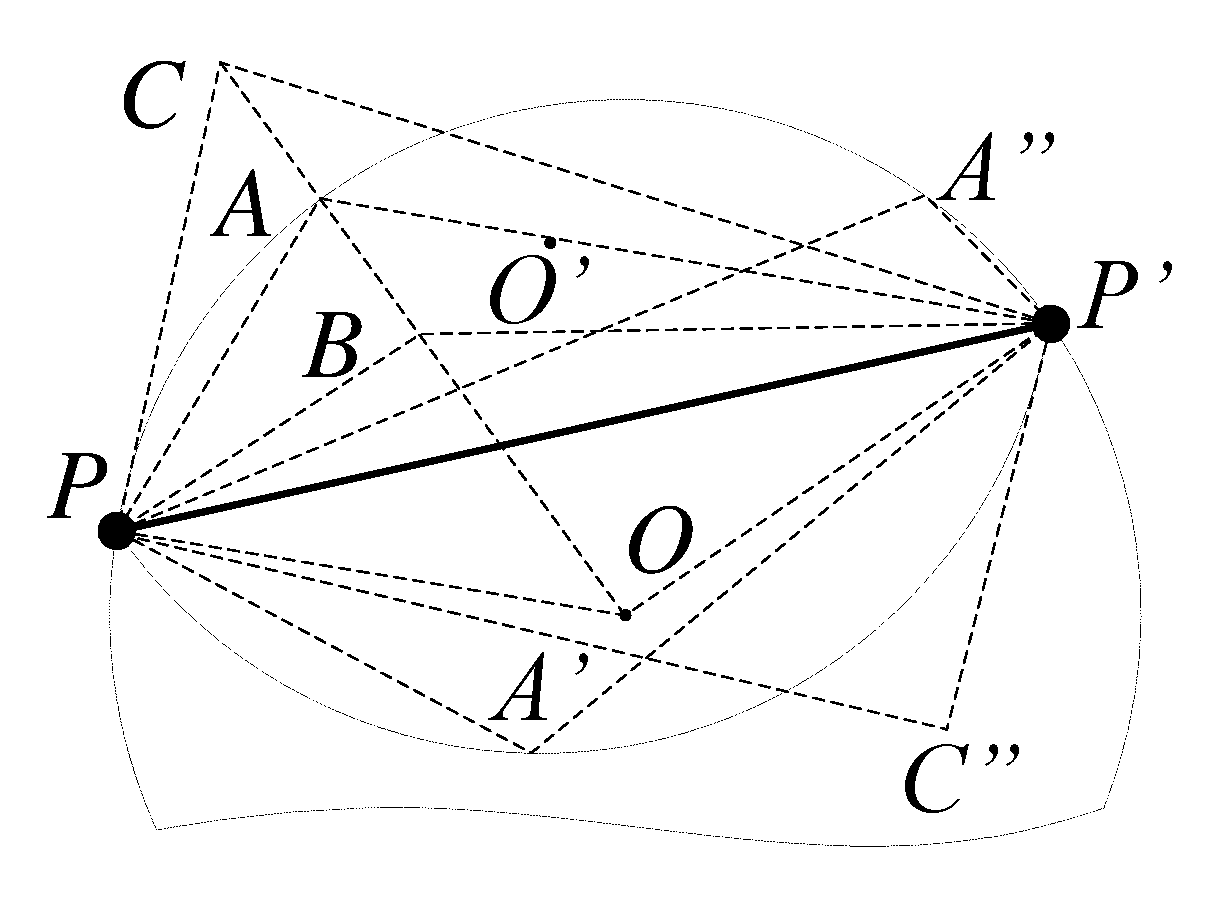
\includegraphics[scale=0.2,keepaspectratio]{InscribedAngle.pdf}
  \caption{Inscribed Angle}
\label{fig:iat}
\end{figure}

We note it due to symmetry, on the other side of line segment $PP'$ we can find another circle center other than $O$ (denoted as $O'$). Its corresponding arc is shown in Fig.~\ref{fig:iat} as arc $PA'P$, and Theorem~\ref{thm:iat} and Corollary~\ref{thm:iatc} also holds to show $\angle PA'P'> \angle PC''P'$. 

Thus we are able to draw the conclusion that for any point namely $B$ located inside the ``olive'' shape $PA'P'A''A$ (which is in fact an \emph{equal-circle-intersection area}), $\angle PBP'> \angle PAP'$; for point $C$ outside this area, $\angle PCP'> \angle PAP'$. Moreover, using analytical geometry techniques, given coordinates of $P$ and $P'$, and the size of $\angle PAP'$, it is not difficult to obtain the coordinates of $O$ and thus determine whether or not a given point is inside the olive area or outside\footnote{The calculation steps are intuitive and thus omitted in this paper.}. We define this procedure as an \textbf{OLIVE.CHK}, which could be used in the \textbf{OLDCAT\_$\mathbf {MT}$} algorithm to find the TURN points. 


\subsubsection{\textbf{OLDCAT\_$\mathbf {MT}$}}
Let's consider $P$ and $P'$ in Fig.~\ref{fig:iat} as two different data points in the raw trajectory data departed by a certain amount of time, and thus there could be a series of other data points taken between them. Theorem~\ref{thm:iat} and Corollary~\ref{thm:iatc} can be used to identify the points where the object makes significant turns (turns with angle sharper than $\Theta_{\rm{min}}$, such as at point $C$ or $C''$), and add them as TURN point to the compressed trajectory $\mathcal P'$. 

In Algorithm~\ref{algo:mt}, once we find a new data point ($P_{t_c}$) which is at least $D_{\rm{max}}$ away from the last data point in the trajectory ($P_{t'}$), we add it to the compressed trajectory ($\mathcal P'$) as a MOVE point, otherwise add to the temporary storage ($\mathcal P_{\rm{temp}}$) as a future candidate of TURN point. 

After adding each MOVE point, the \textbf{while loop} from line 6 to line 16 looks at every data point stored in $\mathcal P_{\rm{temp}}$ and tries to identify TURN points. In every look the data point with earliest time stamp in $\mathcal P_{\rm{temp}}$ is taken out of the storage as $P_{t_A}$. It need three criteria to qualify as a TURN point: 
\begin{itemize}
  \item It is at least $D_{\rm{min}}$ away from $P_{t'}$;
  \item It is at least $D_{\rm{min}}$ away from $P_{t_c}$;
  \item It is located outside the ``olive area'' defined by $P_{t'}$, $P_{t_c}$, and $\Theta_{\rm{min}}$.  
\end{itemize}
Again, the use of $D_{\rm{min}}$ is to tolerate signal noises and errors. 

As discussed in the previous section, a independent procedure \textbf{OLIVE.CHK} uses analytical geometry techniques to confirm whether or not $P_{t_A}$ in outside the olive area, \textit{i.e.} represent a turning angle sharper than $\Theta_{\rm{min}}$. The outline of the procedure is listed in lie 21--28 of Algorithm~\ref{algo:mt}.

\begin{algorithm}
\begin{algorithmic}[1]
\Procedure{\textbf{OLDCAT\_$\mathbf {MT}$}}{$\mathcal P', P_{t_c}, \mathcal P_{\rm{temp}}$}
\State $t'=\max \left\{t|P_t\in \mathcal P'\right\}$
\If{$P_{t'}P_{t_c} > D_{\rm{max}}$}
	\State $P_{t_c} \leftarrow \mathbf M$ \Comment{Add MOVE point}	
	\State $\mathcal P' = \left\{P_{t_c}\right\} \cup \mathcal P'$
	%\State $P = P_{t'}, P' = P_{t_c}$
	\While{$\mathcal P_{\rm{temp}} \neq \emptyset$}
		\State $t_A=\min \left\{t|P_t\in \mathcal P_{\rm{temp}}\right\}$
		%\State $A = P_{t_A}$
		\State $\mathcal P_{\rm{temp}} = \mathcal P_{\rm{temp}} \setminus P_{t_A}$
		\If{\textbf{OLIVE.CHK}$\left(P_{t'}, P_{t_c}, P_{t_A}, \Theta_{\rm{min}}\right)$ \&
			$P_{t'}P_{t_A}, P_{t_A}P_{t_c} > D_{\rm{min}}$}	
			\State $P_{t_A} \leftarrow \mathbf T$	\Comment{Add TURN point}
			\State $\mathcal P' = \left\{P_{t_A}\right\} \cup \mathcal P'$
			\If{${t_A}>t'$}
				\State $P_{t'} = P_{t_A}$
			\EndIf
		\EndIf		
	\EndWhile
\Else
	\State $\mathcal P_{\rm{temp}} = \left\{P_{t_c}\right\} \cup \mathcal P_{\rm{temp}}$
\EndIf
\EndProcedure
\Statex
\Procedure{\textbf{OLIVE.CHK}}{$P, P', A, \Theta_{\rm{min}}$}
	\State Compute coordinates of $O$ and $O'$ 
	\If{$AO<OP$ or $AO<O'P'$}
		\State return FALSE
	\Else 	\State return TRUE
	\EndIf		
\EndProcedure
\end{algorithmic}
\caption{Identifying $\mathbf M$ and $\mathbf T$}
\label{algo:mt}
\end{algorithm}

When we add $P_{t_A}$ as a TURN point in the compressed trajectory $\mathcal P'$, it is possible that ${t_A}>t'$ and $P_{t_A}$ should replace $P_{t'}$ as the last data point in the trajectory before $P_{t_c}$, as done by line 12--14 in Algorithm~\ref{algo:mt}. This is important because for next data points from $\mathcal P_{\rm{temp}}$, the new $P_{t'}$ will be used on line 9 for the distance and olive check. 

We note that with every MOVE point added, data points storage $\mathcal P_{\rm{temp}}$ will be removed one by one (line 8). At the end of the \textbf{while loop}, $\mathcal P_{\rm{temp}}$ should become empty. New data points will be added to $\mathcal P_{\rm{temp}}$ with new \textbf{OLDCAT\_$\mathbf{SBE}$} and \textbf{OLDCAT\_$\mathbf{MT}$} procedures. Thus we could consider $\mathcal P_{\rm{temp}}$ as a ``buffer'' with selected items from the incoming data stream. It is cleared once a MOVE point is added, and will not store the entire history of the collected data points.

The running time complexity of \textbf{OLIVE.CHK} is $O\left(1\right)$. For \textbf{OLDCAT\_$\mathbf{MT}$} it is $O\left(n\right)$, where $n$ is number of data points in $\mathcal P_{\rm{temp}}$. It also needs $O\left(n\right)$ to store $\mathcal P_{\rm{temp}}$. Similar to \textbf{OLDCAT\_$\mathbf{SBE}$}, \textbf{OLDCAT\_$\mathbf{MT}$} does not require all the historic data points to be stored, and is clearly an online algorithm. 

\section{Performance Analysis}
\label{sect:anal}
OLDCAT offers an accuracy for the trajectory data with quality that could be quantified. We show how the error margin could be estimated in Sect.~\ref{sect:acc}. Moreover, OLDCAT is also flexible in adjusting to different application requirements and signal conditions, which will be demonstrated in Sect.~\ref{sect:sca}. 
\subsection{Accuracy and Error Tolerance}
\label{sect:acc}
The accuracy of a trajectory data compression algorithm is determined by the amount of information lost during the compression/sampling process. \emph{Blind spots} are defined as the areas in which the location or direction change of the object may not be detected by the algorithm, and the outcome trajectory $\mathcal P'$ may be inaccurate. For OLDCAT, the ``Olive Area'' between two consecutive data points is its blind spot. 

\begin{figure}[tb]
  \centering
    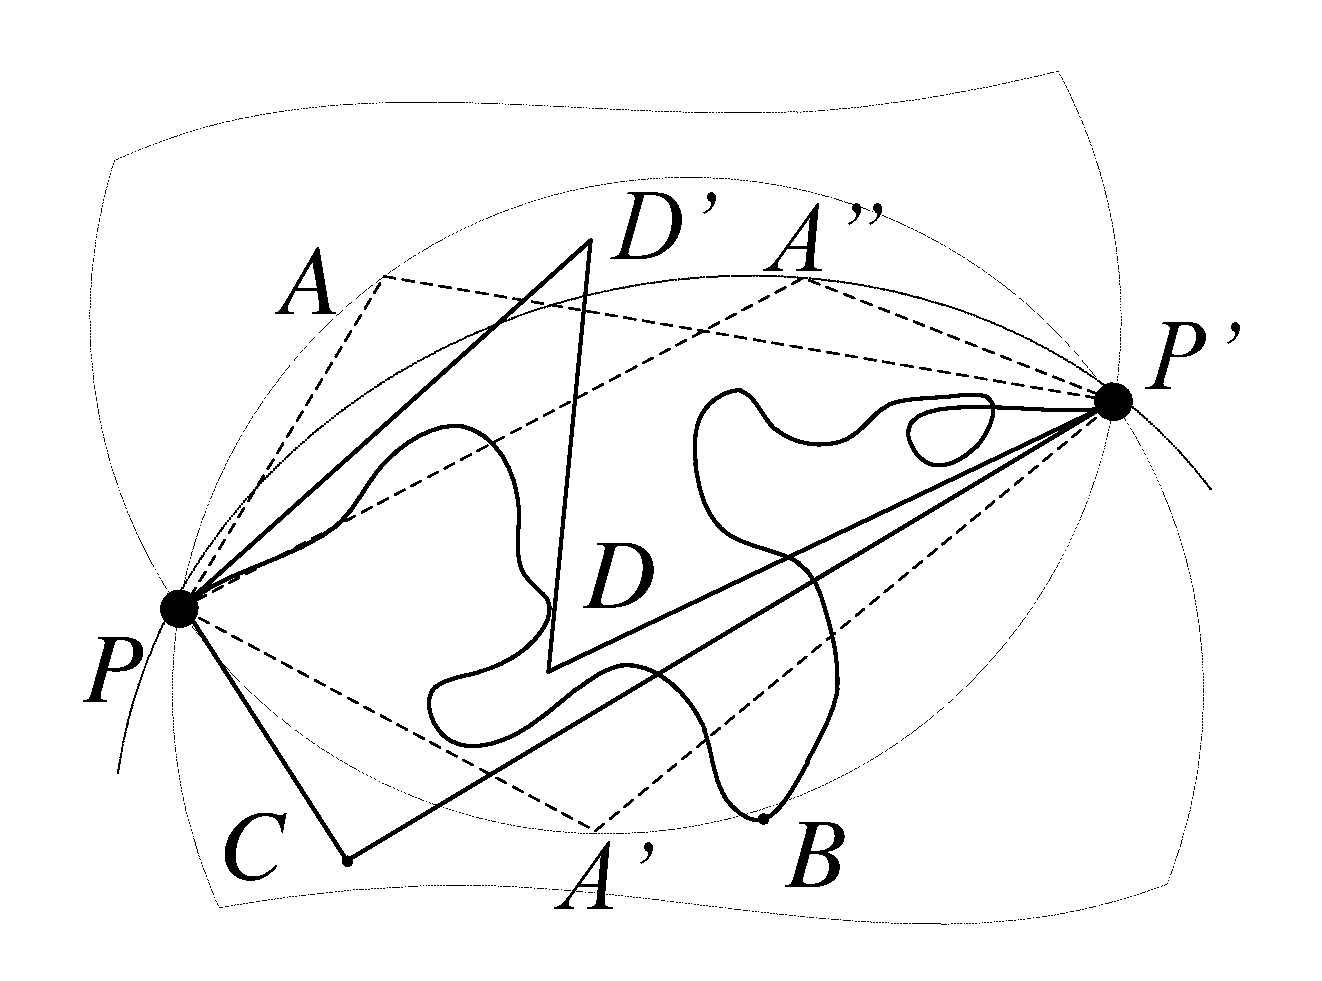
\includegraphics[scale=0.2,keepaspectratio]{BlindSpot.pdf}
  \caption{Blind Spot of OLDCAT}
\label{fig:bs}
\end{figure}

Take Fig.~\ref{fig:bs} as an example. Let's say $P$ and $P'$ are two data points departed by the distance of $D_{\rm{max}}$. The Oliver area could be defined by having $\angle PAP' = \angle PA'P' = \Theta_{\rm{min}}$. While data point $C$ --- outside the blind spot --- could be correctly identified as a TURN point by \textbf{OLDCAT\_$\mathbf{MT}$} procedure, point $D$ and $D'$ will be disregarded, even though the object is making sharper turns at these point, due to the fact that they are located in the blind spot. Similarly, a lot of details of the curvature trace from $P$ to $B$ to $P'$ could be lost since they are in the blind spot. Instead, OLDCAT may compress the trajectory as line segments $PB$ and $BP'$. 

To overcome this, we can reduce $D_{\rm{max}}$ or increase $\Theta_{\rm{min}}$. For example, if we increase $\Theta_{\rm{min}}$ to $\angle PA''P'$, the arc from $P$ to $P'$ will be lower and $D'$ could be identified by \textbf{OLDCAT\_$\mathbf{MT}$} as a TURN point. This is a trade-off between the details of the trajectory and the compression ratio, which will be discussed in the next section. 

With analytical geometry, we could obtain the size of the blind spot (denoted as $\mathbf A_b$) as functions of $D_{\rm{max}}$ (denoted as $d$) and $\Theta_{\rm{min}}$ (denoted as $\theta$):
\[
\mathbf A_b ={d^2}\left( {1 - \frac{\theta }{\pi } - \sin 2\theta } \right){\sec ^2}\theta 
\]

The derivation is simple and thus omitted here. We can see from this equation that $\mathbf A_b $ decreases with  smaller $d$ or larger $\theta$, which seals the conclusion we draw earlier.

Another blind spot is from the $D_{\rm{min}}$ parameter. In both \textbf{OLDCAT\_$\mathbf{SBE}$} and \textbf{OLDCAT\_$\mathbf{MT}$}, we always disregard data points within $D_{\rm{min}}$ from an existing point in $\mathcal P'$. We do this to tolerate the signal noises and errors. 

For example, when the object is stationary, its GPS data could have slight fluctuations. With out the blind area defined by $D_{\rm{min}}$, several STAY point might be identified by \textbf{OLDCAT\_$\mathbf{SBE}$} instead of one. This could add necessary points to the $\mathcal P'$ and thus reduce the efficiency of OLDCAT. 

The $D_{\rm{min}}$ parameter and its drawback is adjustable. If we are confident that the positioning signal is $100\%$ accurate without any noises nor errors, we may set its value to 0 so that the blind spot caused by $D_{\rm{min}}$ will be removed. On the other hand, if the signal and the positioning technique is poor, larger $D_{\rm{min}}$ should be used to tolerate the signal fluctuations, and thus more details of the trajectory will be lost during compression.


\subsection{Scalability and Sensitivity}
\label{sect:sca}
\begin{figure*}[tb] % float placement: (h)ere, page (t)op, page (b)ottom, other (p)age
  \centering{
  \subfloat[Raw Data Points]{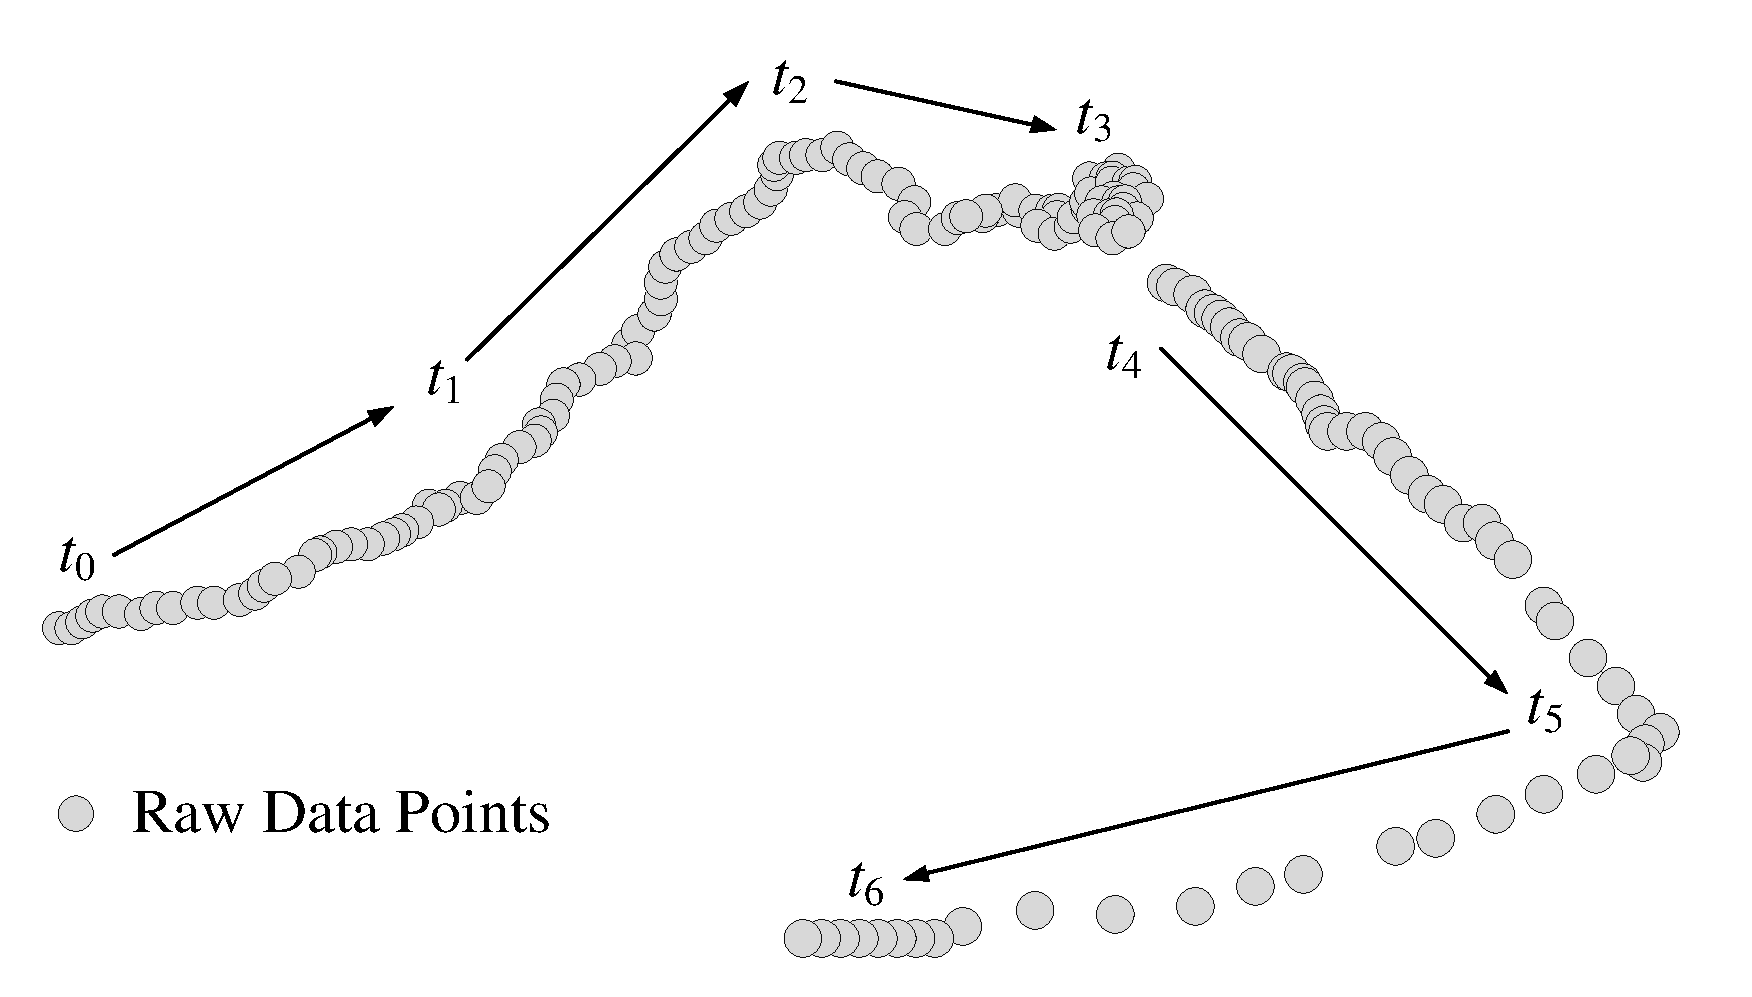
\includegraphics[scale = 0.18,keepaspectratio]{RAW.pdf}
  \label{fig:raw}}
  \subfloat[Reference OLDCAT Trajectory]{ 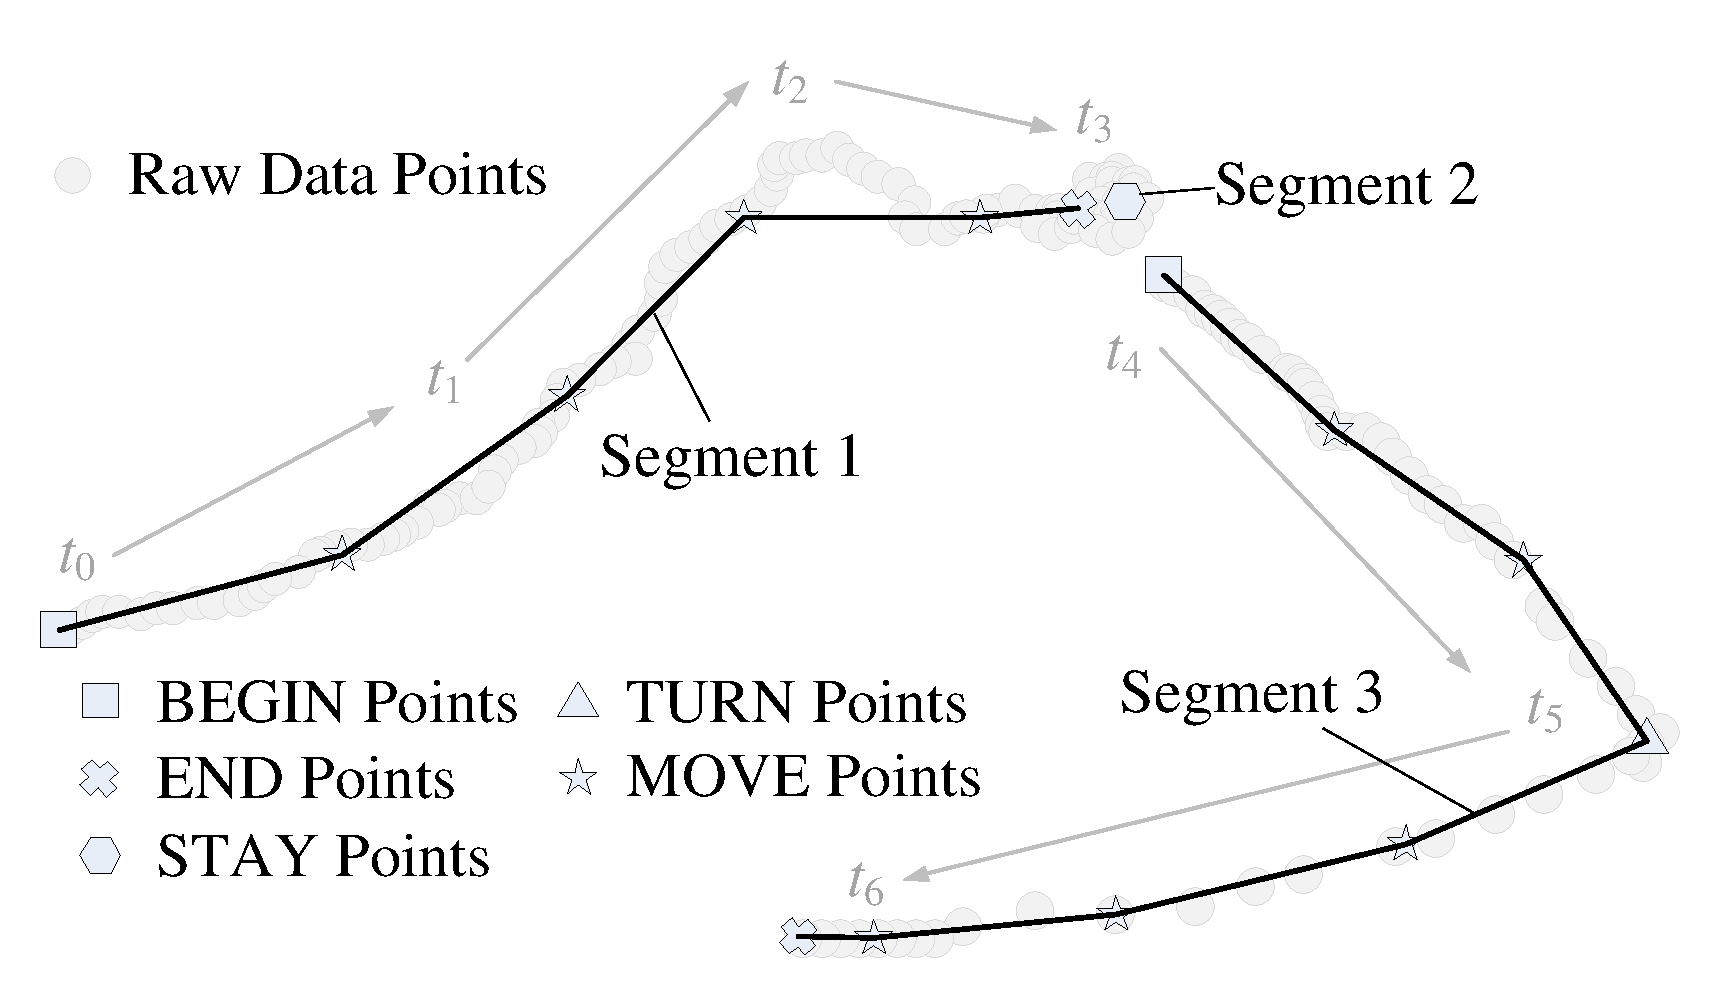
\includegraphics[scale = 0.18,keepaspectratio]{ORIGIN.pdf}\hfill
  \label{fig:ori}}
  \subfloat[$D_{\rm{max}}$ Increases]{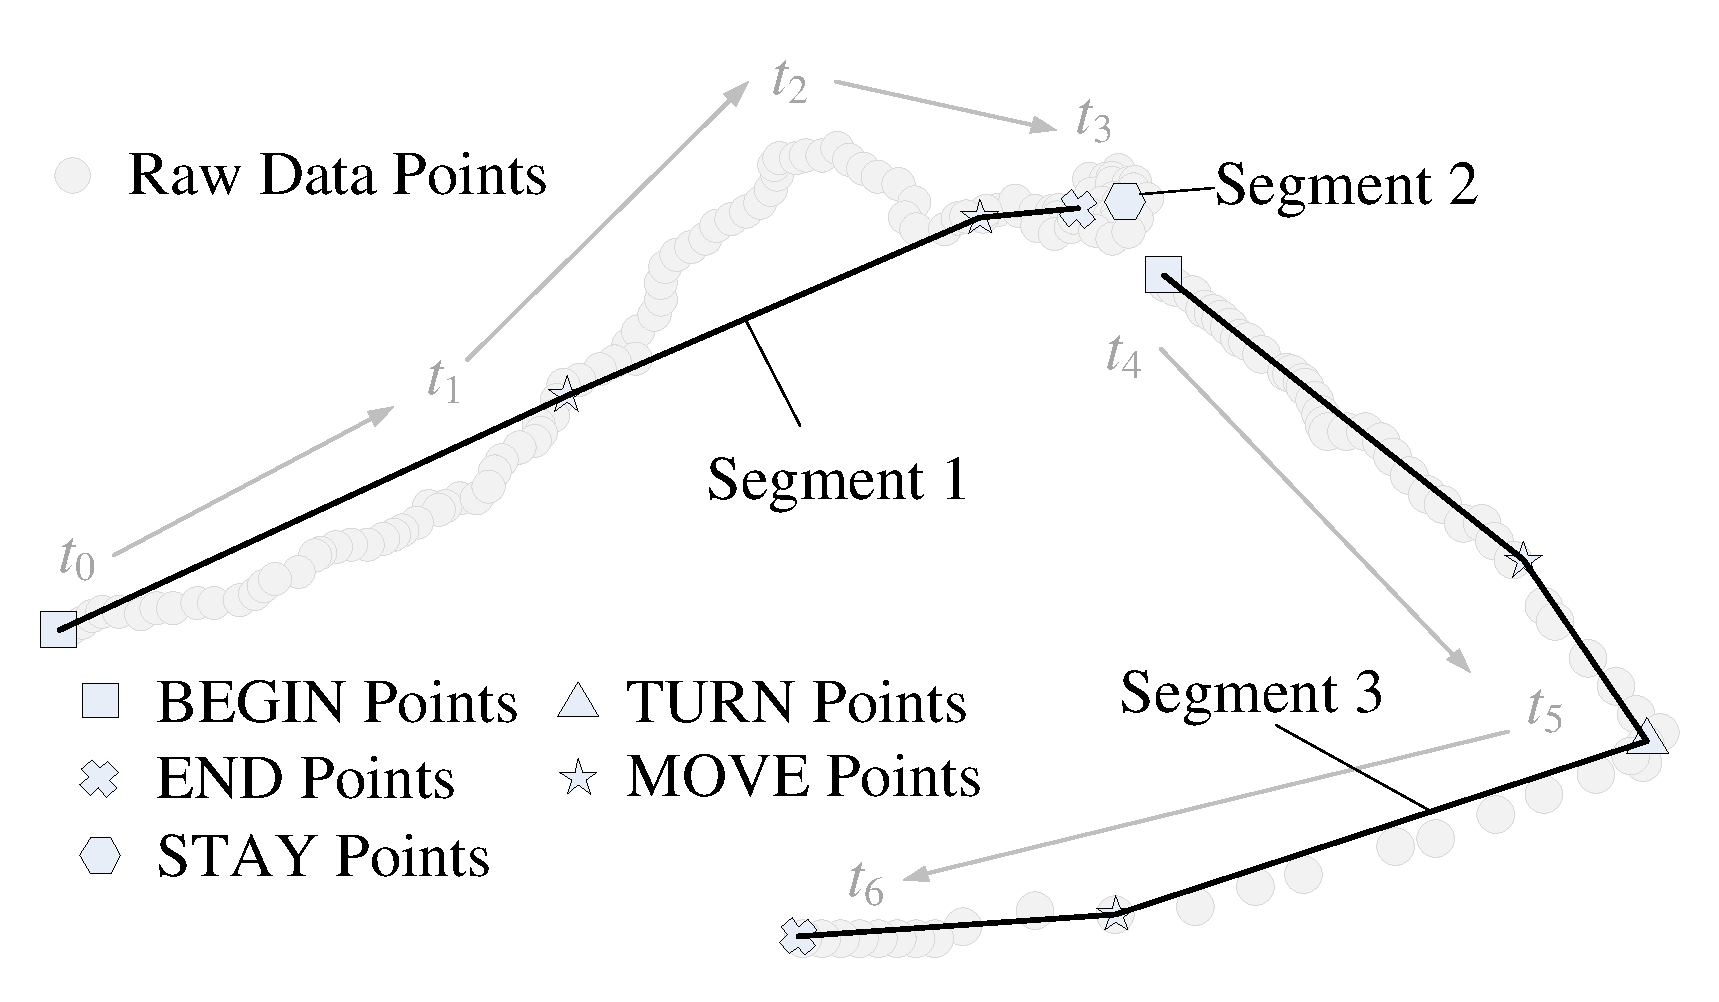
\includegraphics[scale = 0.18,keepaspectratio]{MAXDIST.pdf}\hfill
  \label{fig:maxdist}}\\
  \subfloat[$D_{\rm{min}}$ Decreases]{ 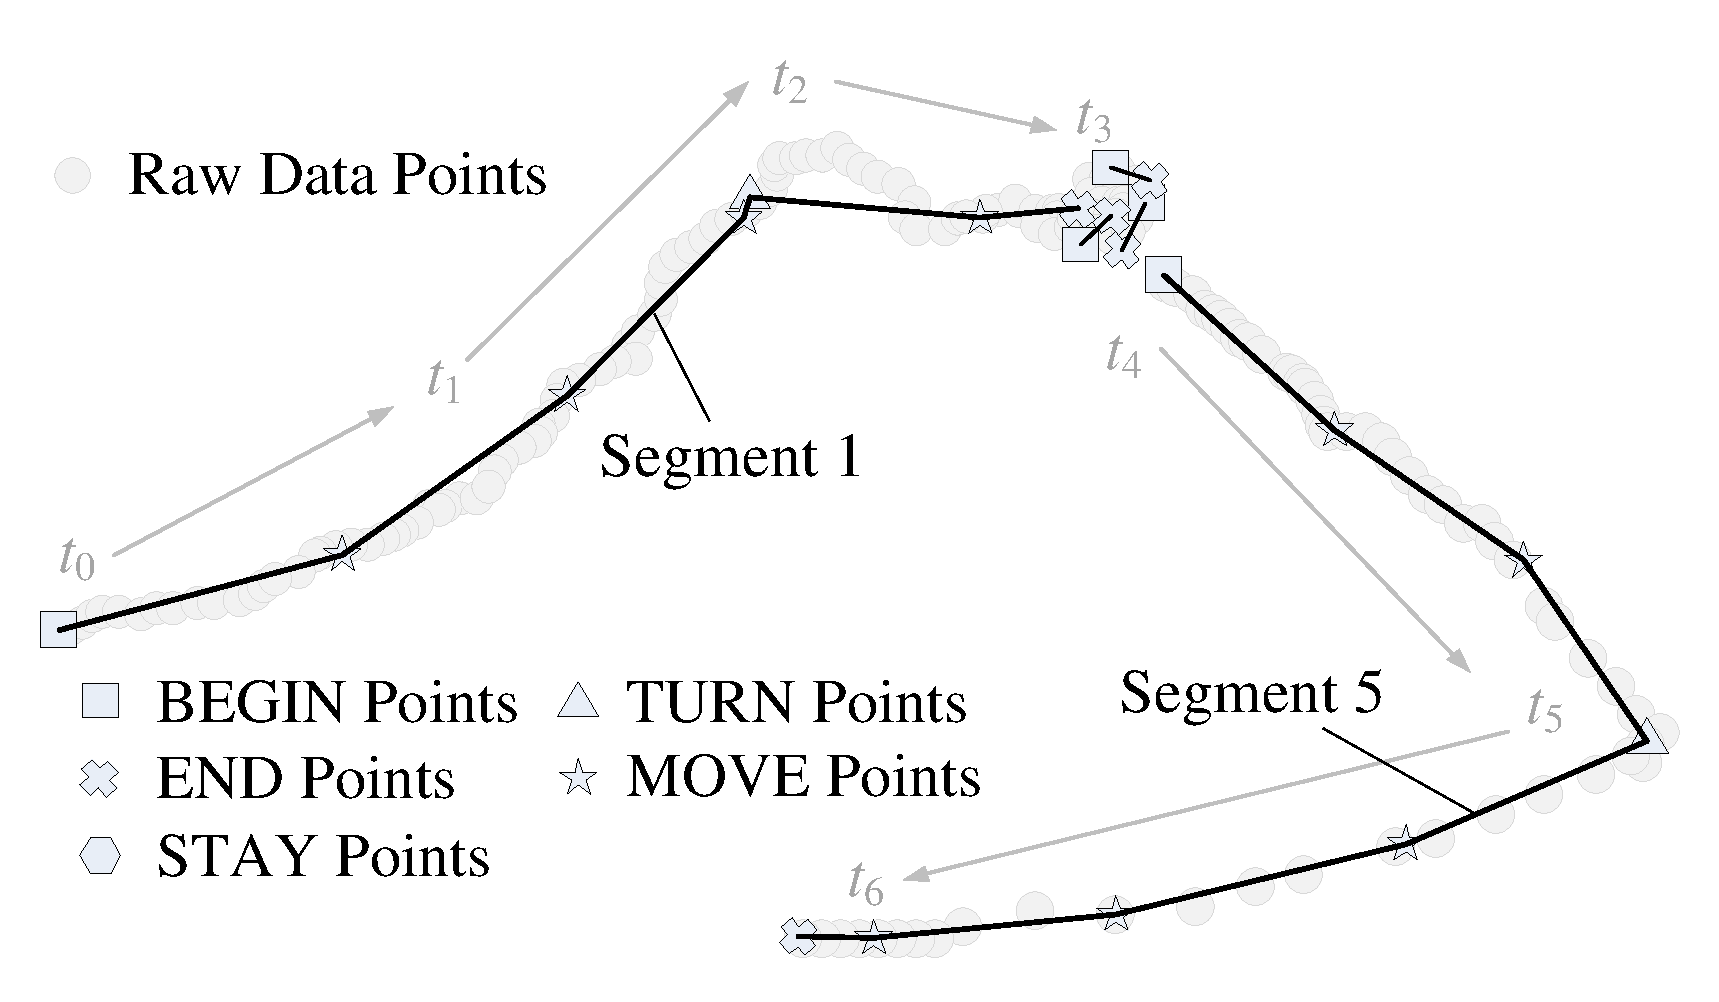
\includegraphics[scale = 0.18,keepaspectratio]{MINDIST.pdf}\hfill
  \label{fig:mindist}}
  \subfloat[$T_{\rm{max}}$ Increases]{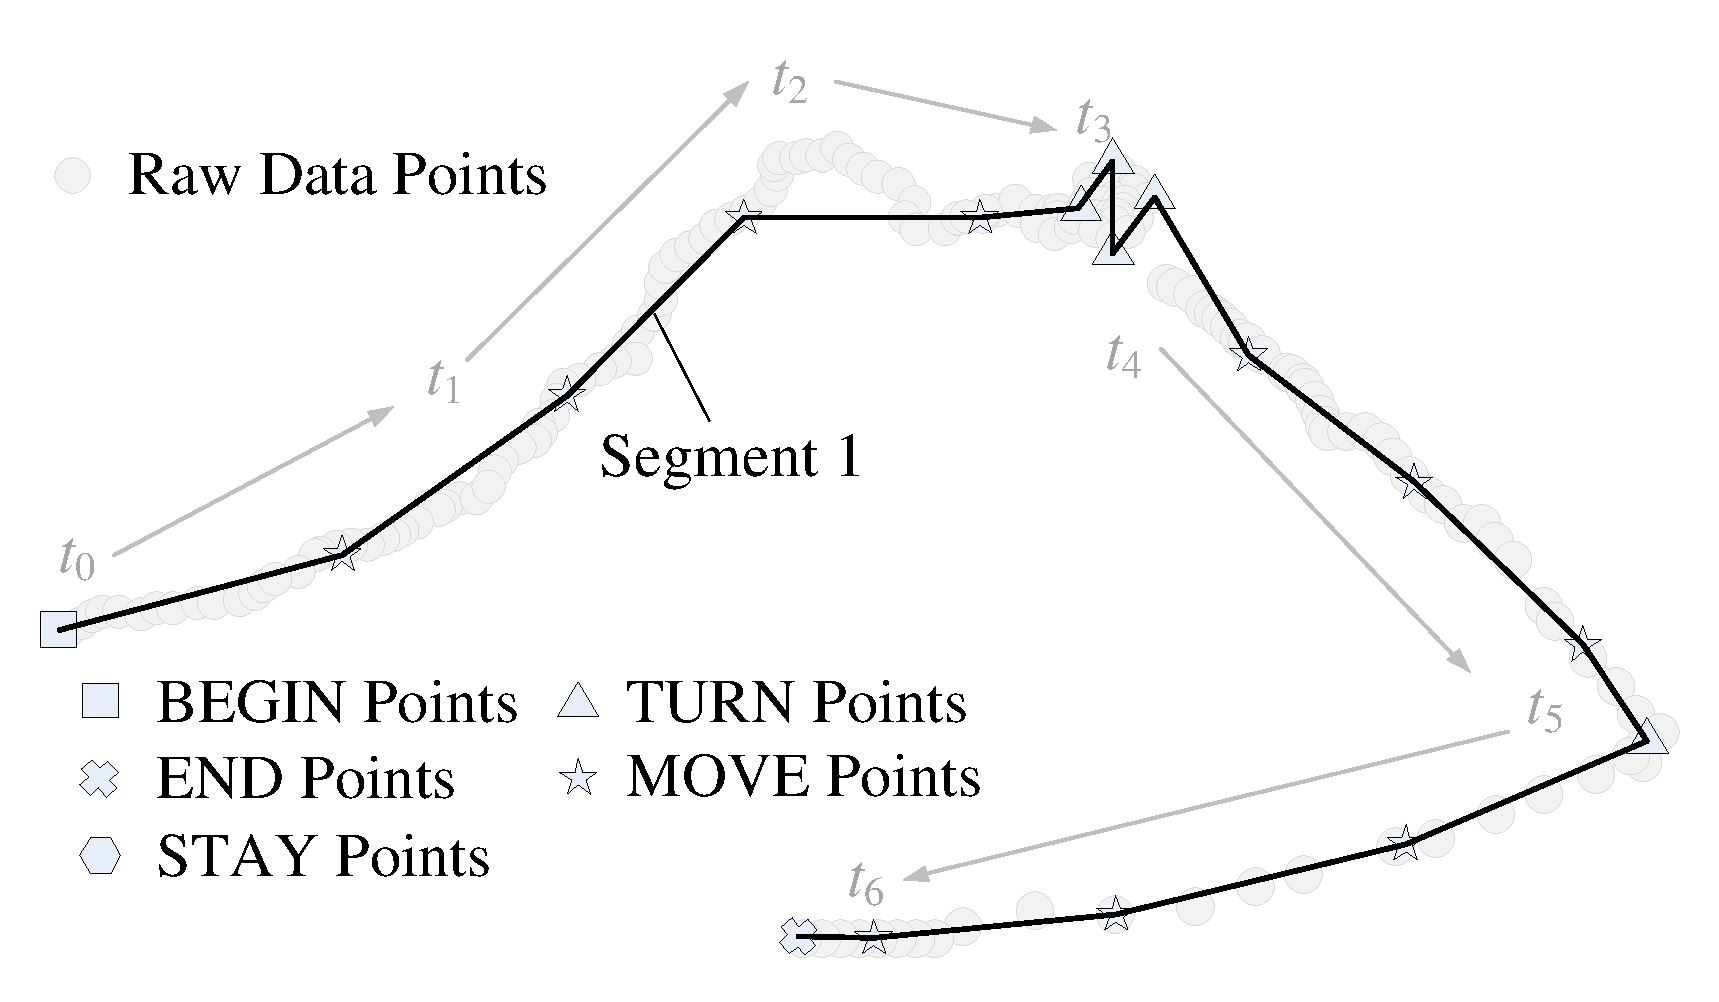
\includegraphics[scale = 0.18,keepaspectratio]{TIME.pdf}\hfill
  \label{fig:time}}
  \subfloat[$\Theta_{\rm{min}}$ Decreases]{ 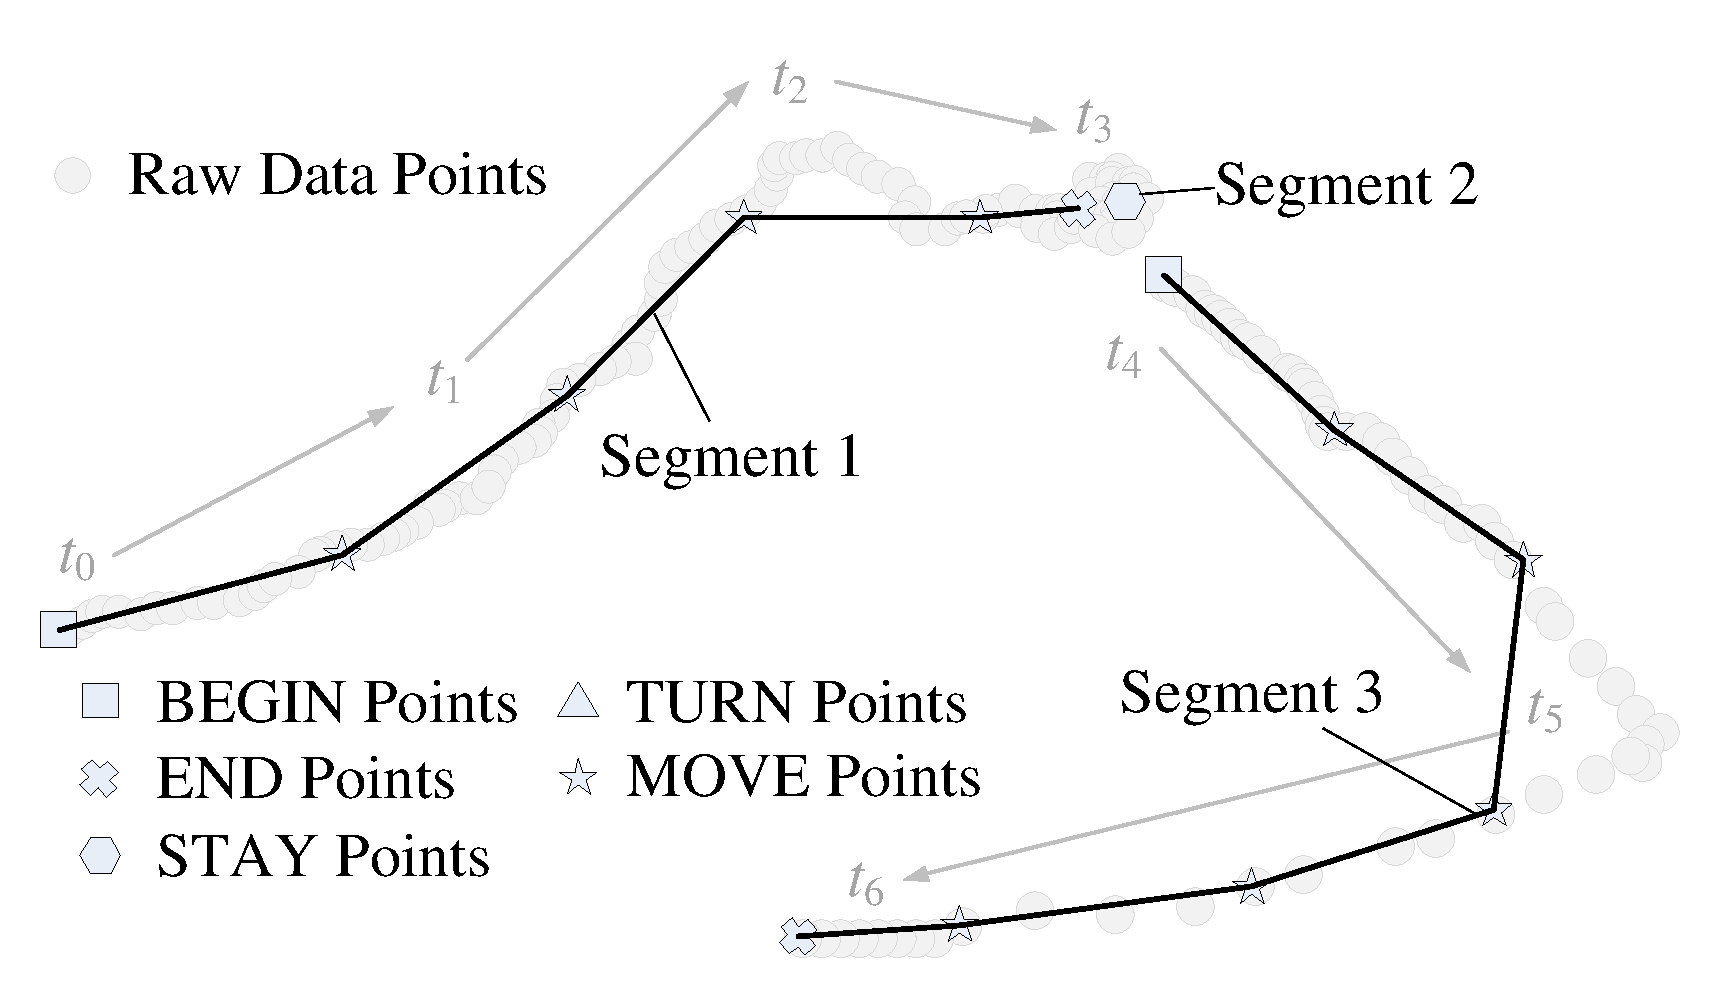
\includegraphics[scale = 0.18,keepaspectratio]{ANGLE.pdf}
  \label{fig:angle}}
  \caption{Changing Parameters in OLDCAT}
  \label{fig:para}}
\end{figure*}
In the previous section we have already shown that the performance of OLDCAT is closely related to its parameters ($D_{\rm{max}}$, $D_{\rm{min}}$, $T_{\rm{max}}$, $\Theta_{\rm{min}}$). In this section with some example and Fig.~\ref{fig:para}, we will show in detail how each of them affects the outcome of OLDCAT.

The Raw trajectory data (before compression) is shown in Fig.~\ref{fig:raw}. We add $t_0$ to $t_6$ to the graph to show the direction of the object's movement. Fig.~\ref{fig:ori} is the reference output of OLDCAT with all the five types of points shown with different notations. A total number of three segments are generated, among which the second segment is of a single STAY point. Fig.~\ref{fig:maxdist} -- \ref{fig:angle} are the outcomes of changing each of the four parameters ($D_{\rm{max}}$, $D_{\rm{min}}$, $T_{\rm{max}}$, $\Theta_{\rm{min}}$), respectively. Comparing them to Fig.~\ref{fig:ori}, we can see the effect of each parameter.

In Fig.~\ref{fig:maxdist} we increase $D_{\rm{max}}$. As a result, only points further away will be added by \textbf{OLDCAT\_$\mathbf{MT}$} as MOVE point. It works fine when the object is moving on a straight course, such as on from $t_4$ to $t_6$ in the figure; but when the object moves on a curvature route, like from $t_0$ to $t_3$, a lot of trajectory details is lost in the compression. Therefore, if we want to retain more details of the trajectory, in particular the curvature, smaller $D_{\rm{max}}$ should be used. 

As we have discussed in the previous section, when we decrease $D_{\rm{min}}$, we lower the noise/error tolerance of OLDCAT. We can see this from Fig.~\ref{fig:mindist}. The STAY point is replaced by three additional very short segments generated between $t_3$ to $t_4$ by \textbf{OLDCAT\_$\mathbf{SBE}$}, and an additional TURN point is identified at about $t_2$ by \textbf{OLDCAT\_$\mathbf{MT}$}. The usefulness of these additional data points is arguable. They could be caused by the signal error and noises and thus ``fake'', but they also could be ``true'' in the sense that a smaller value of $D_{\rm{min}}$ reduces the size of the blind spots, and enables more data points to be added by OLDCAT. No conclusion could be drawn with an actual use case and further knowledge on the positioning signals.

In \textbf{OLDCAT\_$\mathbf{SBE}$}, the value of $T_{\rm{max}}$ determines how we divide the trajectory to  different segments. When its value increases, we wait longer for the next data point in the same segment to show up. From Fig.~\ref{fig:time} we can see that segment 2 and 3 in the original OLDCAT results are now connected to segment 1. This is because with larger value of $T_{\rm{max}}$, the \textbf{if} condition on line 8 of Algorithm~\ref{algo:sbe} becomes more strict, and less points would be considered as BEGIN point. It shows that if we want to study how the trajectory breaks into segments, smaller $T_{\rm{max}}$ value should be used.

We have already shown that a smaller $MAX\_ANGL$ value will cause a larger blind spot, and may miss out potential TURN point. This phenomenon is again shown with Fig.~\ref{fig:angle}. When the value of $MAX\_ANGL$ decreases, the TURN point near $t_5$ disappeared. This makes the compressed trajectory less accurate, but also reduces the number of points in the out come trajectory and hence improves the compression ratio. Adjusting $MAX\_ANGL$ could be effective when we want to show the trajectory in different scales and detail levels. In particular, if we want to study where and how the object makes turns, different values of $MAX\_ANGL$ should be used to give us a more complete picture. 

\section{Case Study with Harbor Data}
\label{sect:case}
Our office is located near the southern shore of Singapore. The Pasir Panjang Container Terminal and Jurong Port lies outside our window. Together, they are one of the busiest port in the world \cite{wpr12}. We have been collecting the \emph{Automatic Identification System (AIS)} signals\footnote{Although heading and speed information are included in AIS signals, we drop them in this study due to their inaccuracy. We also want to test the ability of OLDCAT to deal with minimal given information.} \cite{AIS80} since June 2012. In this study, we are using positioning data of 3000 different ships (randomly sampled out of 3791 in total) over about three weeks time (from 29 June 2012 to 16 July 2012). The data set (\textit{i.e.} $\mathcal P$) has 5708927 lines of records of locations with ship ID and time stamp. Although it is not real time streaming data, we simulated the data stream with stored data when we apply OLDCAT. 

After compress the data using OLDCAT, we obtained 92907 points in $\mathcal P'$. The compression ratio is $1.63\%$. In Fig.~\ref{fig:traj} we show the trajectory obtained by OLDCAT for one single ship and 100 ship respectively. We did not plot the trajectory for all the 3000 ships because the plot is simply overwhelming to make much sense. 

\begin{figure*}[tb] % float placement: (h)ere, page (t)op, page (b)ottom, other (p)age
  \centering{
  \subfloat[Trajectory of One Single Ship]{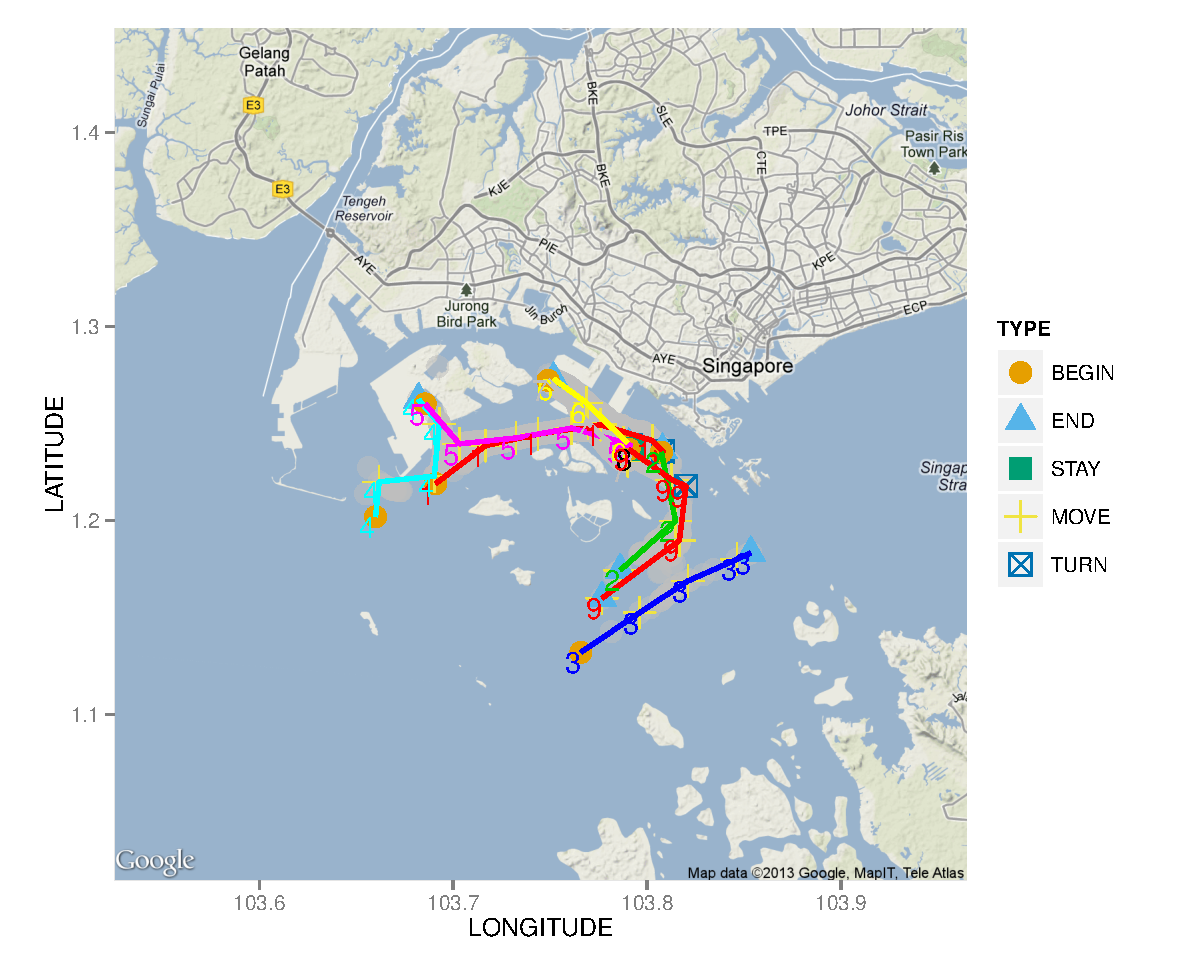
\includegraphics[scale = 0.4,keepaspectratio]{SingleShipMap.pdf}
  \label{fig:1ship}}\hfil
  \subfloat[Trajectory of 100 Ships]{ 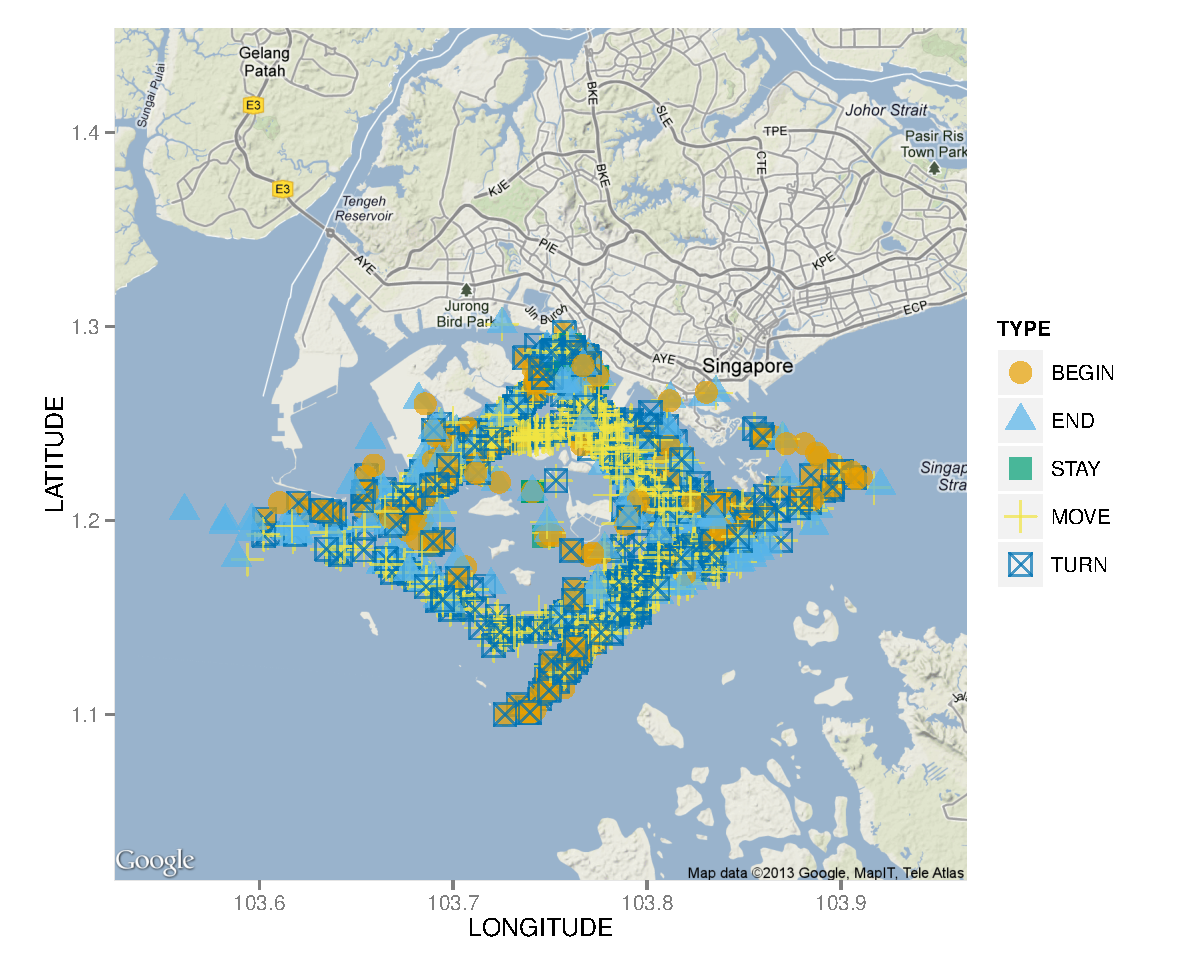
\includegraphics[scale = 0.4,keepaspectratio]{100ShipMap.pdf}
  \label{fig:100ship}}
  \caption{Compressed Trajectory}
  \label{fig:traj}}
\end{figure*}

In Fig.~\ref{fig:1ship}, we can see 9 segments of the ship's trajectory is identified. In particular, we can see how the ship moves into the port in segment 4, then move out in segment 5. Segment 8 is a single STAY point, and is thus less visible in the figure. This plot shows that with as few as $1\%$ of the data points, we can still re-construct the movement of the object, proving the effectiveness of OLDCAT.

Fig.~\ref{fig:100ship} overlays the trajectory of 100 ships. Although due to the high density of the points in the plot, we may not be able to see the sequence of the points, interestingly, we can learn how the ships behave by studying how different types of the points in $\mathcal P'$ distributes over the entire area. For example, a lot of ships make turns at the southern part of the area, indicated by high density of the TURN points (with yellow color), while in the middle they simply keeps moving straight ahead, indicated by the purple color MOVE points. This could be a starting point of studying the behavior and identify regulation violation within the harbor area, which is an interesting extend to the applications of OLDCAT.

\section{Conclusion}
\label{sect:con}
In this paper we propose an \emph{OnLine Data Compression Algorithm for Trajectory (OLDCAT)}. It deals with real time positioning data of moving objects, and tries to identify key characteristic points that defines the trajectory. By taking these points as samples to represent the trajectory, it compress the trajectory data to huge extends. The key strengths of OLDCAT include: online computation, very low ($O\left(n\right)$) running time and storage space complexity, adjustable scale, and signal error/noise tolerance. We have analytically shown the accuracy of the algorithm, and demonstrated examples and use case studies where OLDCAT can effectively compress trajectory data and identify the movement pattern of the objects. 

\bibliographystyle{IEEEtran}
\bibliography{ref}

\begin{IEEEbiography}[{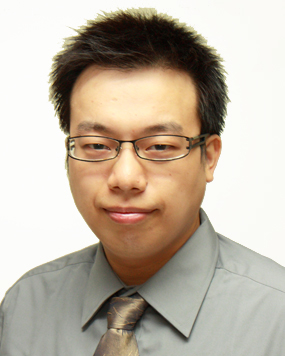
\includegraphics[width=1in,height=1.25in,clip,keepaspectratio]{wt.jpg}}]{Wang Ting}
is born in 1983 in Chengdu, Sichuan, China. He came to Singapore for his undergraduate studies in 2001. He obtained his Bachelor's degree with honors in 2005 and subsequently Ph.D in 2011 both at Nanyang Technological University (NTU), Singapore. 

He worked as a Demand Planner at Apple South Asia and joined SAP as a Data Scientist in 2012. His research interests include data mining, mathematical modeling and algorithmic optimization. 

Dr. Wang loves music and sports. He considers family as his greatest award. He has a son, and he is a good cook --- said his wife.
\end{IEEEbiography}


\end{document}  % This is where a 'short' article might terminate
\balancecolumns

